\section{\textbf{Introduction}}\label{sec:1}
	DC motors are commonly used in robotics due to it's reduced size, light weight and easy velocity control~\cite{CHAPMAN}, avoiding the use of rectifiers or power inverters. In order to change the orientation of a DC motor, for instance, only the direction of the applied voltage needs to change.

	H bridges (see Figure~\ref{fig:bridge}) are simple electronic circuits used to enable a voltage to be applied across a motor in either direction. Despite it's simplicity H bridges might be used to accomplish more challenging tasks, such as stabilizing distributed energy sources~\cite{H-POWER-QUALITY} and improving power quality in electric vehicles~\cite{H-FILTERING}.

\begin{figure}[h]
    \centering
    \centering%
    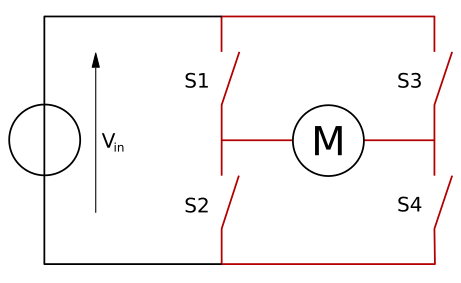
\includegraphics[height=.25\textwidth]{img/H_bridge.png}
    \caption[caption H Bridge]{H Bridge figure borrowed from Wikipedia\protect\footnotemark.}
    \label{fig:bridge}%
\end{figure}
\footnotetext{\url{https://en.wikipedia.org/wiki/H_bridge}}
